% $Header$

\documentclass{beamer}

% This file is a solution template for:

% - Giving a talk on some subject.
% - The talk is between 15min and 45min long.
% - Style is ornate.



% Copyright 2004 by Till Tantau <tantau@users.sourceforge.net>.
%
% In principle, this file can be redistributed and/or modified under
% the terms of the GNU Public License, version 2.
%
% However, this file is supposed to be a template to be modified
% for your own needs. For this reason, if you use this file as a
% template and not specifically distribute it as part of a another
% package/program, I grant the extra permission to freely copy and
% modify this file as you see fit and even to delete this copyright
% notice. 


\mode<presentation>
{
  \usetheme{Berkeley}

  % Code syntax highlighter
  \usepackage{minted}
  
  \usecolortheme{dove}
  % or ...

  \definecolor{mainnetGreen}{rgb}{0.24, 0.68, 0.483} % 

  % \usecolortheme[named=mainnetGreen]{structure}
   \setbeamercolor{palette primary}{bg=mainnetGreen,fg=white}
   \setbeamercolor{palette secondary}{bg=mainnetGreen,fg=white}
   \setbeamercolor{palette tertiary}{bg=mainnetGreen,fg=white}
   \setbeamercolor{palette quaternary}{bg=mainnetGreen,fg=white}


  \setbeamercovered{transparent}
  % or whatever (possibly just delete it)
}


\usepackage[english]{babel}
% or whatever

\usepackage[latin1]{inputenc}
% or whatever


\usepackage{hyperref}
\hypersetup{colorlinks=true,allcolors=blue}

\usepackage[T1]{fontenc}
% Or whatever. Note that the encoding and the font should match. If T1
% does not look nice, try deleting the line with the fontenc.


\title[BlockHack Toronto '23] % (optional, use only with long paper titles)
{Using Bitcoin Cash from mainnet.cash}

\subtitle
{A QuickStart} % (optional)

\author[] % (optional, use only with lots of authors)
{2qx - github.com/2qx}

\date[BlockHack TO] % (optional)
{2023-10-21 10h EDT 
BlockHack Hackathon}

\subject{Using BCH with mainnet.cash}
% This is only inserted into the PDF information catalog. Can be left
% out. 



% If you have a file called "university-logo-filename.xxx", where xxx
% is a graphic format that can be processed by latex or pdflatex,
% resp., then you can add a logo as follows:

% \pgfdeclareimage[height=0.5cm]{university-logo}{university-logo-filename}
% \logo{\pgfuseimage{university-logo}}



% Delete this, if you do not want the table of contents to pop up at
% the beginning of each subsection:
% \AtBeginSubsection[]
% {
%   \begin{frame}<beamer>{Outline}
%     \tableofcontents[currentsection]
%   \end{frame}
% }


% If you wish to uncover everything in a step-wise fashion, uncomment
% the following command: 

%\beamerdefaultoverlayspecification{<+->}


\begin{document}

\begin{frame}
  \titlepage
\end{frame}

\begin{frame}{Outline}
  \tableofcontents
  % You might wish to add the option [pausesections]
\end{frame}


% Since this a solution template for a generic talk, very little can
% be said about how it should be structured. However, the talk length
% of between 15min and 45min and the theme suggest that you stick to
% the following rules:  

% - Exactly two or three sections (other than the summary).
% - At *most* three subsections per section.
% - Talk about 30s to 2min per frame. So there should be between about
%   15 and 30 frames, all told.

\section{Intro}


\subsection[Bitcoin Cash (BCH)]{What is Bitcoin Cash?}

\begin{frame}{bitcoin (cash): a p2p payment network}{with a hidden scripting language}
  % - A title should summarize the slide in an understandable fashion
  %   for anyone how does not follow everything on the slide itself.
  Listen to radio silence.
  \begin{itemize}
    \item
    Rule 1 of Disinformation: Hear no evil, see no evil, speak no evil. Regardless of what you know, don't discuss it -- especially if you are a public figure, news anchor, etc. If it's not reported, it didn't happen, and you never have to deal with the issues.
\item
\href{https://awesomebitcoin.cash/\#whitepaper}{Bitcoin: A Peer-to-Peer Electronic Cash System}
  \end{itemize}
 
\end{frame}




\subsection[Mainnet Cash]{What is Mainnet Cash?}

\begin{frame}{Mainnet Cash is a Specification}{First and foremost.}
  % - A title should summarize the slide in an understandable fashion
  %   for anyone how does not follow everything on the slide itself.

  Mainnet Cash is a tool for developers to access common Bitcoin Cash functions, utilities and the network itself.
  \begin{itemize}
  \item
    A written contract for how a service will be provided.
  \item
    Implemented in typescript.
  \item
    Specified in OpenAPI3 (Swagger): \href{https://rest-unstable.mainnet.cash/api-docs/}{api.yml}
    \item
    A generated API is then implemented with the typescript library.
    
  \end{itemize}
\end{frame}

\begin{frame}{Visual Explanation}{}
  % - A title should summarize the slide in an understandable fashion
  %   for anyone how does not follow everything on the slide itself.

  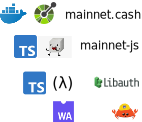
\includegraphics[width=0.6\textwidth, angle=0]{stack.pdf}
\end{frame}


\begin{frame}{mainnet.cash is wasm wrapped in typescript, then candied, cured with REST \& shipped with docker}{}
  % - A title should summarize the slide in an understandable fashion
  %   for anyone how does not follow everything on the slide itself.

  
  \begin{itemize}
  \item
    \href{https://libauth.org/}{@bitauth/libauth} functional bitcoin library.
  \item
    mainnet-js: defacto reference wallet implementation. 
  \item
    mainnet.cash an API specification implemented with mainnet-js.
    \item
        End Goal:
        \begin{itemize}
        \item
        Developers can use common BCH functions from REST.
        \item
        Developers get a similar interface in the browser. 
        \end{itemize}
  \end{itemize}
  
\end{frame}
\subsection[Batteries included]{What's in the box?}

\begin{frame}{Other tools included}{-}
  % - A title should summarize the slide in an understandable fashion
  %   for anyone how does not follow everything on the slide itself.
  \begin{itemize}
    \item
      Automatic network providers for different networks (bitcoincash, chipnet, regtest)
    \item
      \href{https://github.com/bitjson/cashtokens}{CashTokens} \& \href{https://github.com/bitjson/chip-bcmr}{BitcoinCash Metadata Registries (BCMR)} built in.
    \item
      BIP39/BIP44 Mnemonic seed wallets and xpub derivation.   
    \item
      Caching interface to the CoinGecko USD spot API.
    \item
      Available plugin for \href{https://cashscript.org/}{CashScript}.
    \item
      Available storage plugins for browsers (IndexedDB) or nodejs (postgres)
    \end{itemize}
\end{frame}


\begin{frame}{RE: mainnet.cash is a contract}{}
  % - A title should summarize the slide in an understandable fashion
  %   for anyone how does not follow everything on the slide itself.

  \includegraphics[width=1\textwidth, angle=0]{python_perp.png}
\end{frame}



\section{Ways to use mainnet-js}

\subsection[Javascript]{Running mainnet-js Bundled Script}

\begin{frame}[fragile]
    \frametitle{Run the packages from a Browser}
    When developing from a \href{https://jsfiddle.net/bdqujn25/}{jsfiddle} or codepen...

    
    \rule{\textwidth}{0.4pt}
    \tiny
    \begin{minted}{html}
<!-- mainnet-js -->
<head>
  <script src="https://cdn.mainnet.cash/mainnet-2.2.5.js"
   integrity="sha384-RrFMKtXQroWNZV6mP8XFAV2FOIFsEPSAfzd5e7V1H1qSnLg8wwO2bkLb5URNOv+k"
   crossorigin="anonymous"></script>
</head>
    \end{minted}
\rule{\textwidth}{0.4pt}
\end{frame}


\begin{frame}[fragile]
    \frametitle{Get the answer}
    Using a plain text file and firefox
    \rule{\textwidth}{0.4pt}
    {\fontsize{3pt}{3.6pt}\selectfont
    \begin{minted}{html}
      
<!DOCTYPE html>
<html>
<head>
    <script src="https://cdn.mainnet.cash/mainnet-2.2.5.js"
   integrity="sha384-RrFMKtXQroWNZV6mP8XFAV2FOIFsEPSAfzd5e7V1H1qSnLg8wwO2bkLb5URNOv+k"
   crossorigin="anonymous"></script>
     <script src="https://cdn.mainnet.cash/contract/contract-2.2.5.js"
 integrity="sha384-0+mqq/sJ3NSWb6rJWjkNirr8TvHU3dEJyHvHmm1ZfNVytR32mGDZnh+2EiDQUcvc"
 crossorigin="anonymous"></script>
     <script>
script=`
pragma cashscript ^0.8.0;

contract LifeTheUniverseAndEverything() {
    function get_answer(int answer) {
        require(answer==42);
    }
}
`
    document.addEventListener("DOMContentLoaded", async (event) => {
        globalThis.exports = globalThis.exports || {};
            Object.assign(globalThis, await __mainnetPromise);
            Object.assign(globalThis, await __contractPromise);

        let a = new Contract(script, []);
        console.log(await a.getDepositAddress());
        console.log(await a.getUtxos());
        console.log(await a.getBalance());
        //let getAnswer = a.getContractFunction("get_answer")
        //console.log(await getAnswer(42n).to("bitcoincash:qqad5sy4jml3f6vcp246dulsex04xp48wq23d35rqe", 1000n).send())
    });
    </script>     
</head>
<body>
</body>
</html>
    \end{minted}
    }
\rule{\textwidth}{0.4pt}
\end{frame}


\begin{frame}[fragile]
    \frametitle{Do you want to develop an app?}
    we have the webapps...
    \begin{itemize}
      \item
        \href{https://github.com/mainnet-cash/mainnet-js/tree/master/demo/vue-nuxt}{Demo Folder}.
        \item
        libauth, and now mainnet-js are ESM modules.
        \item
        Expect there to be a slight issue with top-level awaits.
        \item
        Tree shaking is possible, but no on our end.
        \item
        If you get a working configuration in the hip new web framework, consider a PR to the demo list.
      \end{itemize}
        
\rule{\textwidth}{0.4pt}
\end{frame}

\subsection[Unstable REST]{Using mainnet.cash service}

\begin{frame}[fragile]
  \frametitle{Try a demo version of mainnet.cash REST}
    from REST
  \rule{\textwidth}{0.4pt}
  \tiny
  \begin{minted}{shell}
    
# Verify a signed message via REST
curl -X 'POST' \
  'https://rest-unstable.mainnet.cash/wallet/signed/verify' \
  -H 'accept: application/json' \
  -H 'Content-Type: application/json' \
  -d '{
  "walletId": "watch:mainnet:qqad5sy4jml3f6vcp246dulsex04xp48wq23d35rqe",
  "message": "2qx#72497 lucky_guava_52595 discord",
  "signature": 
  "H+O9Oz+9FFdaA9UCzTidbVh0CvWcrGduTRFCQnDifEKVRz3Fk1KFyZa88XSLmfGAVB/glP8OFRJqSatZtzo8h9I="
}'

  \end{minted}
\rule{\textwidth}{0.6pt}
\end{frame}

\subsection[Docker image]{Using the mainnet.cash Docker image}

\begin{frame}[fragile]
    \frametitle{Starting your own mainnet.cash}
      To start your own mainnet.cash REST service
    \rule{\textwidth}{0.9pt}
    \tiny
    \begin{minted}{shell}
# get the image from docker
docker pull mainnet/mainnet-rest

# start the image, with one process, 
# exposing locally at 3000 to the container's port 80
# & pass it details of the regression configuration
docker run -d --name Mainnet --env WORKERS=1 \ 
            -p 127.0.0.1:3000:80 \ 
            --env-file .env.regtest \
            mainnet/mainnet-rest
    \end{minted}
\rule{\textwidth}{0.9pt}

\end{frame}

\begin{frame}[fragile]
    \frametitle{Stopping your own mainnet.cash}
      Just in case something \alert{goes wrong}...
    \rule{\textwidth}{0.6pt}
    \tiny
    \begin{minted}{shell}
# checking logs, to find the issue
docker logs -f Mainnet

# restarting, stopping, forcefully stopping.
docker restart Mainnet
docker stop Mainnet
docker kill Mainnet

# if your machine is paging memory or sounds like a jet plane
sudo killall node 
# kills all docker processes
docker stop $(docker ps -a -q)
    \end{minted}
\rule{\textwidth}{0.6pt}
assuming your container was given the name "Mainnet".\\
\end{frame}

\begin{frame}[fragile]
    \frametitle{More Usage Samples and Configuration Information}
  % Keep the summary *very short*.
  \begin{itemize}
    \item
      There's more at: \href{https://mainnet.cash/tutorial/running-rest.html}{mainnet.cash/tutorial/running-rest.html}
    \item
      Including a full list of \href{https://mainnet.cash/tutorial/running-rest.html#configuration}{configuration variables.}
    \item
      This is an \href{https://rest-unstable.mainnet.cash/api-docs/}{unstable public instance} of the REST service for testing and educational purposes
    \end{itemize}
        
\rule{\textwidth}{0.9pt}
\end{frame}

\subsection[RegTest Stack]{Spin-up a Full Service Stack in Regtest}

\begin{frame}[fragile]
    \frametitle{Running a RegTest Stack}
      The mainnet-js source code contains a full RegTest Stack, deployed with docker compose.
    \rule{\textwidth}{0.6pt}
    \tiny
    \begin{minted}{shell}

#  To start a regtest stack,
# from the mainnet-js source directory...
yarn regtest:up

# reset everything
yarn regtest:down; yarn regtest:up
    \end{minted}
\rule{\textwidth}{0.6pt}
There's more in the \href{http://mainnet.cash/tutorial/#regtest-wallets}{docs}.\\


Having your own private networks allow for better tests, testing in time, testing with a RegTest Bitcoin Cash chain. \\ 
Note: the docker images for the stack took about 6 min to download over wifi.
\end{frame}

\begin{frame}[fragile]
    \frametitle{The RegTest Secrets}
    One of the advantages of RegTest is reusing and sharing secrets  
    \rule{\textwidth}{0.4pt}
    \tiny
    \begin{minted}{javascript}
ADDRESS="bchreg:qpttdv3qg2usm4nm7talhxhl05mlhms3ys43u76rn0"
ADDRESS_TOKEN="bchreg:zpttdv3qg2usm4nm7talhxhl05mlhms3ysjm0q59vu"
ADDRESS_LEGACY="18uVyRcvE7RdR9WFLyD1kMPjehKxyE91in"
PRIVATE_WIF="cNfsPtqN2bMRS7vH5qd8tR8GMvgXyL5BjnGAKgZ8DYEiCrCCQcP6"
ALICE_ID="wif:regtest:cNfsPtqN2bMRS7vH5qd8tR8GMvgXyL5BjnGAKgZ8DYEiCrCCQcP6"
BOB_ID="seed:regtest:divide battle bulb improve hockey favorite charge save merit fatal frog cage:m/44'/0'/0'/0/0"

    \end{minted}
\rule{\textwidth}{0.4pt}
\end{frame}

\section{Warning}

\subsection[Not the way]{Nothing is impossible, it's just not the way}

\begin{frame}[fragile]
  \frametitle{mainnet-js currently needs wasm}

  Webassembly is currently a core requirement, given the state of libauth.  This 
  means the only enviornments where mainnet-js can't be used are places that can't satisfiy that requirement.
% Keep the summary *very short*.
\begin{itemize}
  \item
    webassembly is \alert{NOT} supported in React Native,
  \item
    ... because Google, Apple and Meta. 
    \item
    Mainnet-js also won't work with \href{https://caniuse.com/wasm}{IE, Opera Mini or KaiOS 2.5}
  \end{itemize}
      
\rule{\textwidth}{0.9pt}
\end{frame}


\begin{frame}[fragile]
  \frametitle{browser wallets}

  Not every user has your browser.
% Keep the summary *very short*.
\begin{itemize}
  \item
    Be very careful expecting a user's browser to have persistent storage.
  \item
    Consider the cross-browser experience, wallet recovery, potentual loss of seed and funds if browser storage doesn't persist.
  \end{itemize}
      
\rule{\textwidth}{0.9pt}
\end{frame}


\section{Manuals}
\begin{frame}{Where to get more information}
  Where to get more infprmation
  % Keep the summary *very short*.
  \begin{itemize}
  \item
     \href{https://mainnet.cash/tutorial/}{Javascript walk-thrus at for mainnet-js}
  \item
    Correlate  \href{https://mainnet.cash/tutorial/rest.html}{walk-thrus for the REST service} 
  \item
    Demo \href{https://github.com/mainnet-cash/mainnet-js/tree/master/demo}{webapp configurations}
  \item
    mainnet.cash \href{https://rest-unstable.mainnet.cash}{Swagger REST interface}
  \item
    Every feature should also have test coverage, if/when documation is incomplete.
  \item
    If you graduate to libauth, remember the reference implementation.
  \end{itemize}
  \end{frame}



%%%%%%%%%%%%%%%%%%%%%%%%%%%%%%%%%%%%%%%%%%%%%%%%%%
%%%%%%%%%%%%%%%%%%%%%%%%%%%%%%%%%%%%%%%%%%%%%%%%%%
%%%%%%%%%%%%%%%%%%%%%%%%%%%%%%%%%%%%%%%%%%%%%%%%%%

\section{State of mainnet.cash}

\begin{frame}{Committed to Adoption}
Mainnet Cash is built to last, but...
% Keep the summary *very short*.
\begin{itemize}
\item
    The project is in a \alert{stable alpha}. 
    \item
    libauth v2 is also (technically) in alpha.
\item
    Currently in a \alert{feature freeze}.
\item
    Seeking \alert{broader adoption}, and usage.
\item
    An independent \alert{security audit} needed before warnings are removed.
\end{itemize}
\end{frame}

\begin{frame}{Committed to Adoption}
  That said\dots

  \begin{itemize}  
\item
mainnet.cash (REST API) handled roughly \$2.2T of transactions in 2021 as the BCH backend software for noise.cash.
\item
Used for early prototyping of \href{https://old.hop.cash}{early hop.cash} and \href{https://selene.cash}{selene.cash}.
\item
Used by the \href{https://cashonize.com/}{Cashonize} CashToken web wallet.
\item
Used extensively for regression testing of \href{https://www.npmjs.com/package/@unspent/phi}{unspent/*}.
\item
Second library to market for CashTokens and first BCMR library to market (?).
\item
Mainnet.cash is almost three years old in javascript land.
\end{itemize}
\end{frame}

\begin{frame}{The Future}

Mainnet Cash was built to be maintained.
% The following outlook is optional.
\vskip0pt plus.5fill

% Keep the summary *very short*.
\begin{itemize}
\item
    Really conservative and maintenance oriented design choices from the start.
\item
    Extensive investment in testing and a testing harness
\item
    These values are also apparent in supporting libraries.
\end{itemize}


\begin{itemize}
\item
    Outlook
    \begin{itemize}
    \item
    \alert{@bitauth/libauth} has a nice upgrade in the works.
    \end{itemize}
\end{itemize}
\end{frame}

\begin{frame}{Contact}

    
    % The following outlook is optional.
    \vskip0pt plus.5fill
    
    % Keep the summary *very short*.
    \begin{itemize}

       \item More documentation at \href{https://mainnet.cash/}{mainnet.cash}
       \item Please report \href{https://github.com/mainnet-cash/mainnet-js/issues}{Bugs on Github}.
       \item Join our \href{https://t.me/mainnetcash}{ mainnet.cash Telegram Channel} for support.
    \end{itemize}

\end{frame}

\begin{frame}{Any Questions?}{}
  % - A title should summarize the slide in an understandable fashion
  %   for anyone how does not follow everything on the slide itself.

  \includegraphics[width=0.6\textwidth, angle=0]{pumpkins.jpeg}
\end{frame}

\end{document}

